\documentclass{article}
\usepackage{graphicx}
\usepackage{ffcode}
\usepackage[utf8]{inputenc}

\title{IDATT2202 OBL1-OS}
\author{Nicolai H. Brand}
\date{September 2022}

\begin{document}

\maketitle

\section{}
\subsection{}
    The program is copied into memory. The stack and heap space are allocated by the kernel. The kernel sets the instruction pointer to the first instruction and starts executing. Before the execution properly happens, the kernel switches the processor from kernel- to user-mode. This is because a user made/user download program does not have access to the same functionality and privilege levels that the kernel has. This is one of many measures taken by the kernel to ensure security and reliability. 

\subsection{}
    a) the $pid\_t pid$ member of the $task\_struct$ stores the process ID.\\
    b) There is a variable $acct\_vm\_mem1$ og type unsigned 64 (long) that stores accumulated virtual memory usage.
    
    I am assuming a field means a member of a struct. For example, the struct members $void *stack$ points to beginning of the stack for the process. $unsigned int flags$ holds a bunch of flags that describe some metadata about the process. 

\section{}
\subsection{}
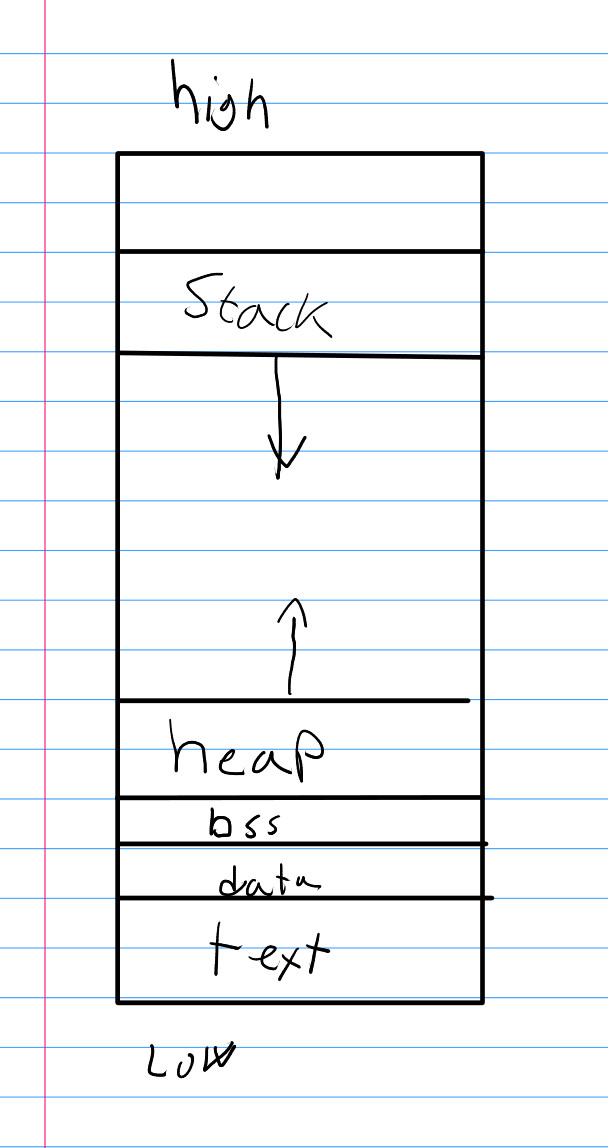
\includegraphics[width=50mm,scale=0.5]{address_space.jpg}

\subsection{}
The code segment is actually a part of the text segment, and some sources even omit the code segment altogether and just refers to it as a part of the text segment. The code + text segment stores the the programs' execution instructions. The data segment includes the bss segment and stores global and staticly defined variables. The heap stores dynamically allocated memory for the program. The stack stores local memory for the program. Each new function call gets its own stack.

Address $0x0$ is unavailable is it represents null. Any pointer type can points here when its address/reference is set to the NULL identifier.

\subsection{}
In C, a global variable is available everywhere inside a program. It is not tied to a specific function or scope (other than the global scope). A static variable is only initialized once and is persistent until program execution ends. A local variable is tied to a specific scope, usually block scope or lexical scope, and is removed when it goes out of scope. It is therefore only available inside the scope it was declared. 

$var1$ is on the data segment as it is declared outside a function and has global scope. 

$var2$ is on the stack as it has local scope since it is declared inside the scope of the $main$ function. 

$var3$ is also on the stack, but it points to allocated memory on the heap.

\section{}
\subsection{}
Using the GNU size I find that the size of text is 1695 bytes, data is 600 bytes and bss is 8 bytes. 

\subsection{}
Running objdump –f on the binary returns gives the start address $0x0000000000001060$.

\subsection{}
The name of the function at the start address is $\_start$. The $\_start$ function is the entry point of any C program. It contains the startup code for the C runtime environment. 

\subsection{}
This is because the kernel does address randomization. This is done for security reasons. If the address were constants, it could be leveraged by malicious software. 

\section{}
\subsection{}

\subsection{}
Running ulimit -s returns $8192$ meaning I have a default stack size of $8 MiB$.

\subsection{}
The program has infinite recursion with no way to break out of it. When a function is called, the kernel creates a new stack for the function. The program crashes because it uses up all the available stack memory since no stacks are freed while new ones keep piling up on eachother.

\subsection{}
This result of the command gives how many times the function recursed (called itself). On my system I get around $500,000$ function calls before it crashes.

\subsection{}
The default stack on my machine has about $8192 * 10^3$ bytes of space. Running $stackoverlow.c$ crashes after around $500,000$ recursively function calls. This gives:

$$ \frac{8192 * 10^3}{5 / 2 * 10^5} = \frac{8192 * 2}{5 * 10^2} ~= 32 bytes $$

Every stack frame takes up about $32$ bytes.
\end{document}
